%
% dinupa3@gmail.com
% 04-13-2023
%

\documentclass[12pt, xcolor={dvipsnames}, aspectratio = 169, sans,mathserif]{beamer}

\usepackage{fontspec}
\usepackage{fontawesome5}
\usepackage{mathrsfs}
\usepackage{amsmath}
\usepackage{graphicx}
\usepackage{hyperref}
\usepackage[absolute,overlay]{textpos}
\usepackage[font=tiny]{caption}


\mode<presentation>
{
\usefonttheme{serif}
% \setmainfont{OpenDyslexicAlta NF}
\definecolor{nmsured}{RGB}{137,18,22} % custom colors
\setbeamercolor{title}{fg=White,bg=nmsured}
\setbeamercolor{frametitle}{fg=White,bg=nmsured}
\setbeamercolor{section number projected}{bg=nmsured,fg=White}
\setbeamercolor{subsection number projected}{bg=nmsured,fg=White}
\setbeamertemplate{items}{\color{nmsured}{$\blacksquare$}}
\setbeamertemplate{section in toc}[square]
\setbeamertemplate{subsection in toc}[square]
\setbeamertemplate{footline}[frame number]
\setbeamertemplate{caption}[numbered]
\setbeamerfont{footnote}{size=\tiny}
\setbeamercovered{invisible}
\usefonttheme{professionalfonts}
%\setbeamertemplate{background}[grid][color=nmsured!15] % set background
\setbeamertemplate{navigation symbols}{} % remove navigation buttons
}

\title{ORR Meeting: Hodoscope \& NIM Trigger Subsystem}
\author{SpinQuest/E1039 Collaboration}

%
% some custom commands
%
\newenvironment{List}[2]
{
\begin{textblock}{#1}#2
\begin{itemize}
}
{
\end{itemize}
\end{textblock}
}

\newenvironment{Pic}[2]
{
\begin{textblock}{#1} #2
\begin{figure}
}
{
\end{figure}
\end{textblock}
}

%
%
%
\begin{document}

%
%
\begin{frame}
  \maketitle
\end{frame}

%
%
\begin{frame}[fragile]{Hodoscope \& NIM Trigger Subsystem}
\begin{Pic}{10.0}{(0.5, 2.0)}
  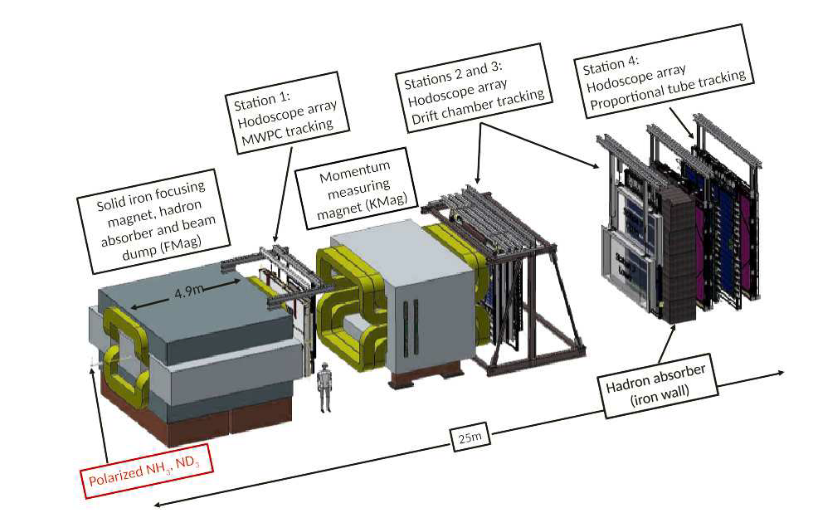
\includegraphics[width=10.0cm]{imgs/spectrometer.png}
  \caption{SpinQuest/E1039 spectrometer.}
\end{Pic}

\begin{List}{5.0}{(10., 2.5)}

  \item We have four hodoscope stations in the SpinQuest/E1039 spectrometer.

  \item We name them as \verb|H1, H2, H3, H4|.

\end{List}

\end{frame}

\begin{frame}[fragile]{Hodoscope \& NIM Trigger Subsystem}
\begin{List}{15.0}{(0.5, 2.5)}

  \item We are currently using five NIM trigger system for cosmic ray tracking.

  \begin{verbatim}
  NIM1: a 4 fold trigger -> H1 and H2 and H3 and H4
  NIM2: a 2 fold trigger -> H1 and H2
  NIM3: a random trigger
  NIM4: a 2 fold trigger -> H2 and H4
  MATRIX5: a 2 fold trigger -> (H1 and H2) or (H2 and H4)
  \end{verbatim}

  \item Timing adjustment in \verb|MATRIX5| is reverse beam-like.

  \item RF timing is included in \verb|NIM1|, \verb|NIM2| and \verb|NIM4| triggers.

\end{List}
\end{frame}

\begin{frame}
\begin{Pic}{15.0}{(0.5, 0.5)}
  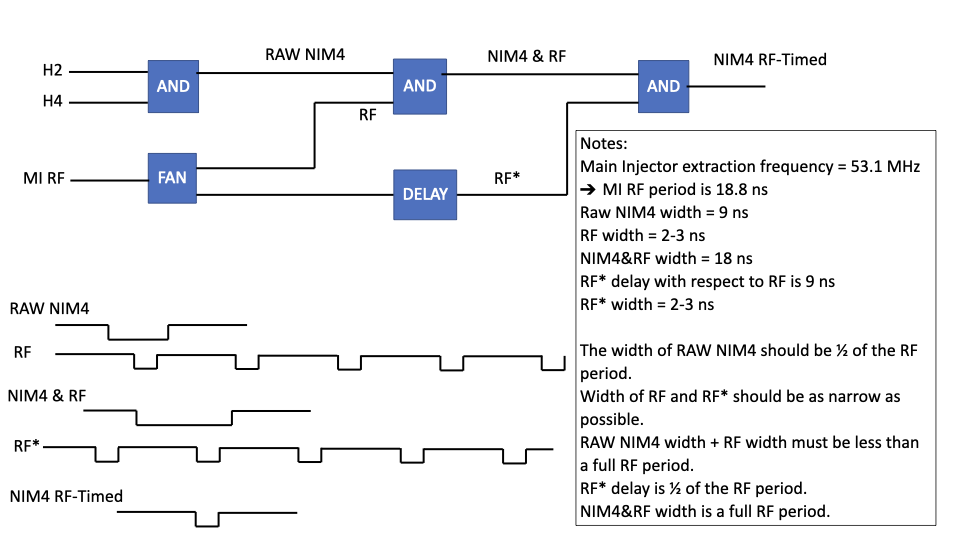
\includegraphics[width=13.0cm]{imgs/rf_timing.png}
  \caption{Trigger logic diagram used for RF timed trigger. Credit S. Pate.}
\end{Pic}
\end{frame}

\begin{frame}[fragile]{Hardware and Electronics}
\begin{List}{5.0}{(0.5, 2.5)}

  \item We are currently maintaining a 20\% of the spare \verb|NIM/CAMAC|  modules for beam time.

  \item We have setup a test bench for electronic module testing.
\end{List}

\begin{Pic}{10.}{(6., 2.5)}
  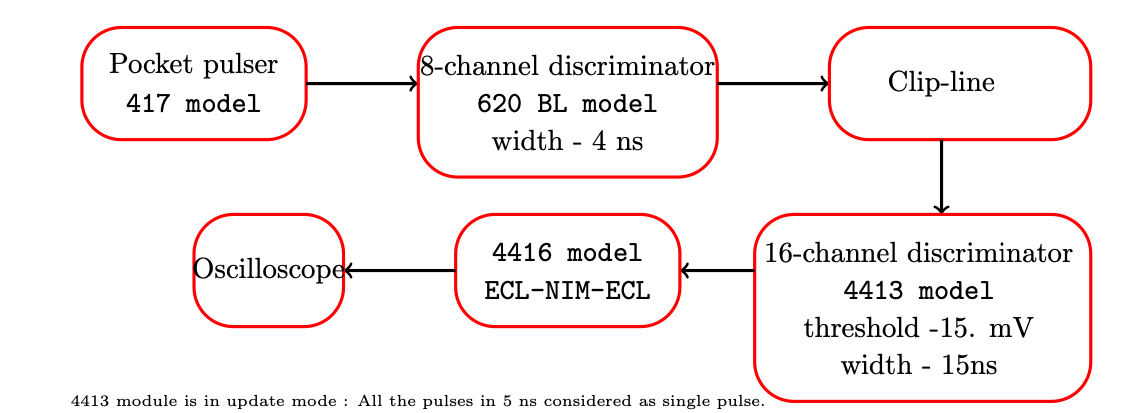
\includegraphics[width=10.0cm]{imgs/test_bench.png}
  \caption{Block diagram of the test bench set up.}
\end{Pic}

\end{frame}

\begin{frame}[fragile]{Hodoscope Efficiencies}
\begin{List}{15.0}{(0.5, 2.5)}

  \item We use \verb|NIM2| and \verb|NIM4| triggers to calculate the hodoscope efficiencies.

  \item We use runs taken from 04-03-2023 to 04-09-2023 days.

\end{List}
\end{frame}

\begin{frame}{Hodoscope Efficiencies}
\begin{Pic}{15.}{(0.5, 2.5)}
  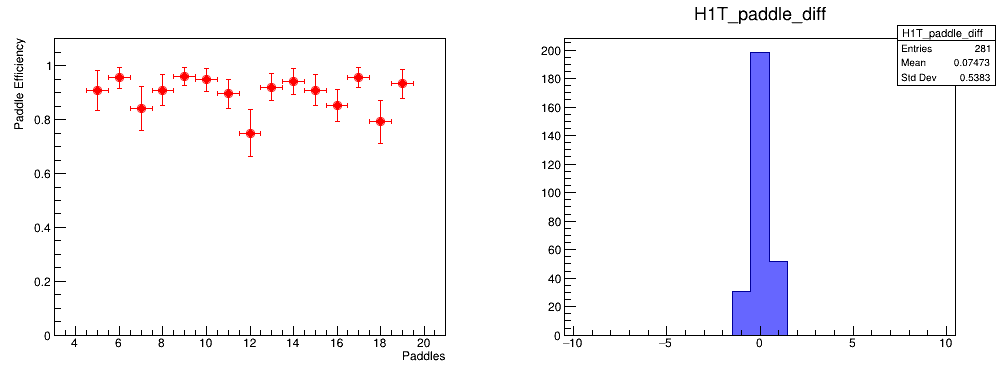
\includegraphics[width=15.0cm]{imgs/H1T_paddle_diff.png}
  \caption{H1T paddle efficiency.}
\end{Pic}
\end{frame}

\begin{frame}{Hodoscope Efficiencies}
\begin{Pic}{15.}{(0.5, 2.5)}
  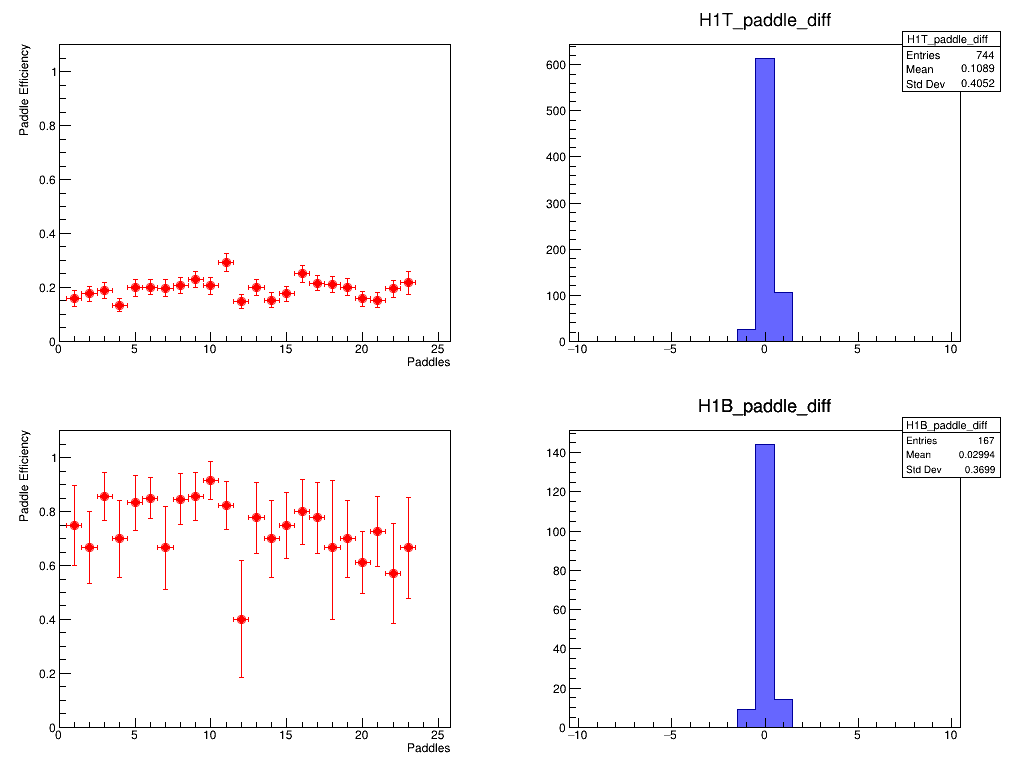
\includegraphics[width=15.0cm]{imgs/H1B_paddle_diff.png}
  \caption{H1B paddle efficiency.}
\end{Pic}

\begin{List}{15.0}{(0.5, 11.)}
  \item Due to the angle of the detector it is hard to get good tracks in this plane. But this is issue will be resolved with beam.
\end{List}
\end{frame}

\begin{frame}{Hodoscope Efficiencies}
\begin{Pic}{15.}{(0.5, 2.5)}
  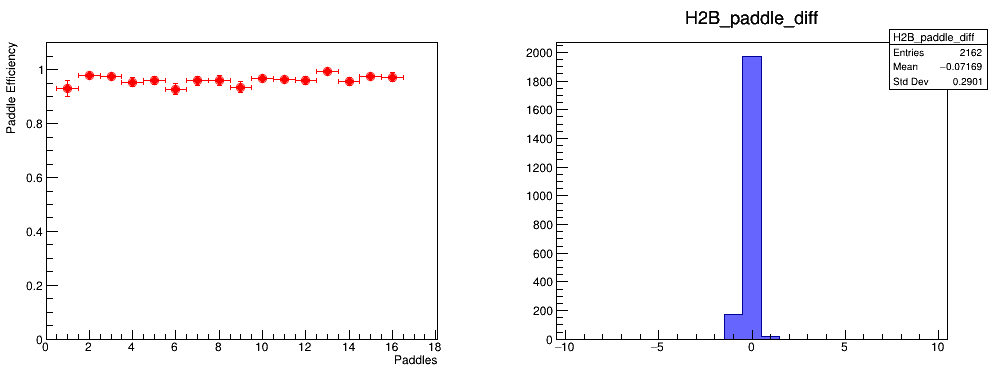
\includegraphics[width=15.0cm]{imgs/H2B_paddle_diff.png}
  \caption{H1B paddle efficiency.}
\end{Pic}
\end{frame}

\begin{frame}{Hodoscope Efficiencies}
\begin{Pic}{15.}{(0.5, 2.5)}
  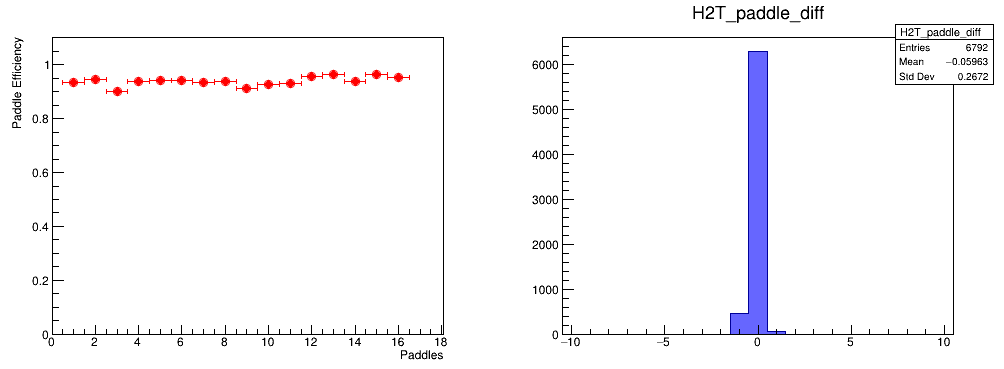
\includegraphics[width=15.0cm]{imgs/H2T_paddle_diff.png}
  \caption{H2T paddle efficiency.}
\end{Pic}
\end{frame}

\begin{frame}{Hodoscope Efficiencies}
\begin{Pic}{15.}{(0.5, 2.5)}
  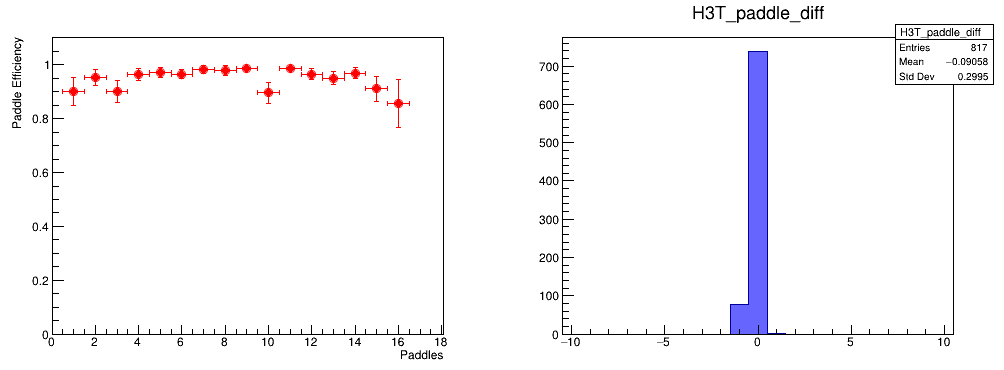
\includegraphics[width=15.0cm]{imgs/H3T_paddle_diff.png}
  \caption{H3T paddle efficiency.}
\end{Pic}
\end{frame}

\begin{frame}{Hodoscope Efficiencies}
\begin{Pic}{15.}{(0.5, 2.5)}
  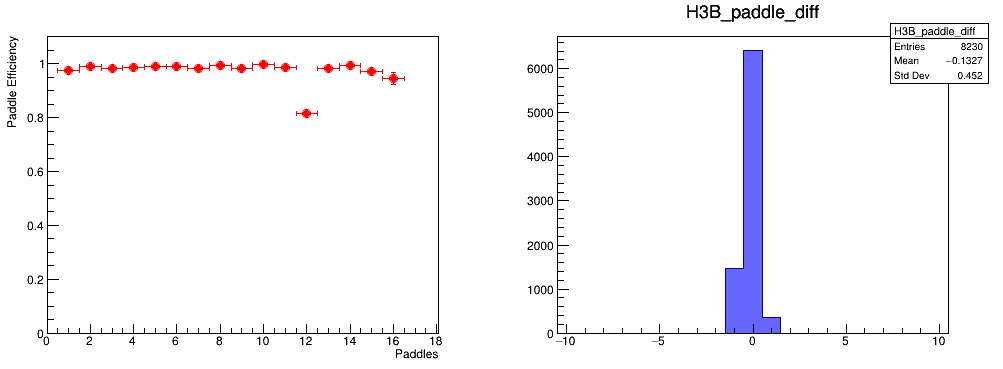
\includegraphics[width=15.0cm]{imgs/H3B_paddle_diff.png}
  \caption{H3B paddle efficiency.}
\end{Pic}
\end{frame}

\begin{frame}{Hodoscope Efficiencies}
\begin{Pic}{15.}{(0.5, 2.5)}
  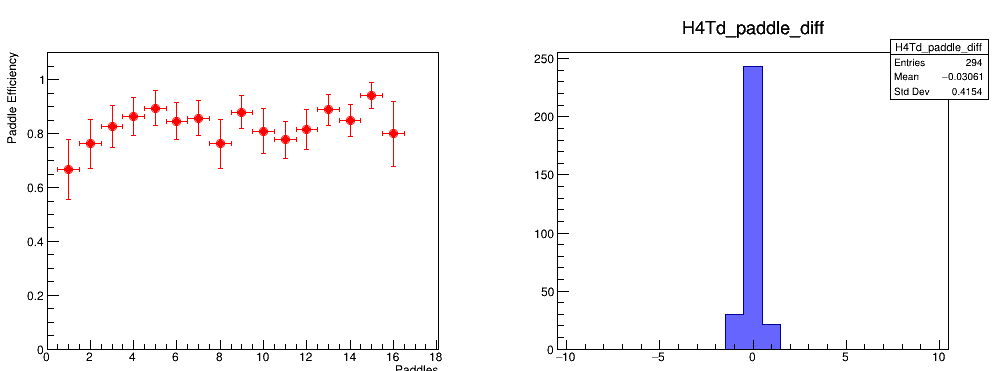
\includegraphics[width=15.0cm]{imgs/H4Td_paddle_diff.png}
  \caption{H4Td paddle efficiency.}
\end{Pic}
\end{frame}

\begin{frame}{Hodoscope Efficiencies}
\begin{Pic}{15.}{(0.5, 2.5)}
  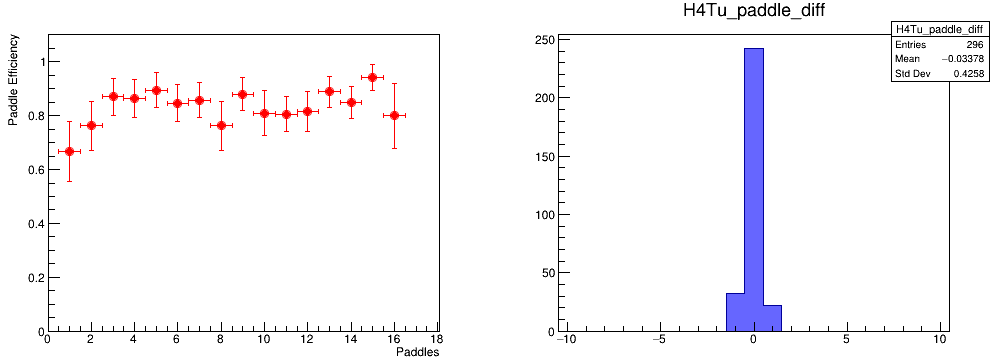
\includegraphics[width=15.0cm]{imgs/H4Tu_paddle_diff.png}
  \caption{H4Tu paddle efficiency.}
\end{Pic}
\end{frame}

\begin{frame}[fragile]{Monitoring the Hodoscope Subsystem Remotely}
\begin{List}{5.0}{(0.5, 2.5)}

  \item We have prepared a GUI/CL tools to easy debugging the hodoscopes without accessing the experimental hall.

  \item This tool will be useful during the beam-time to debug hodoscope.

\end{List}

\begin{Pic}{10.}{(6., 2.5)}
  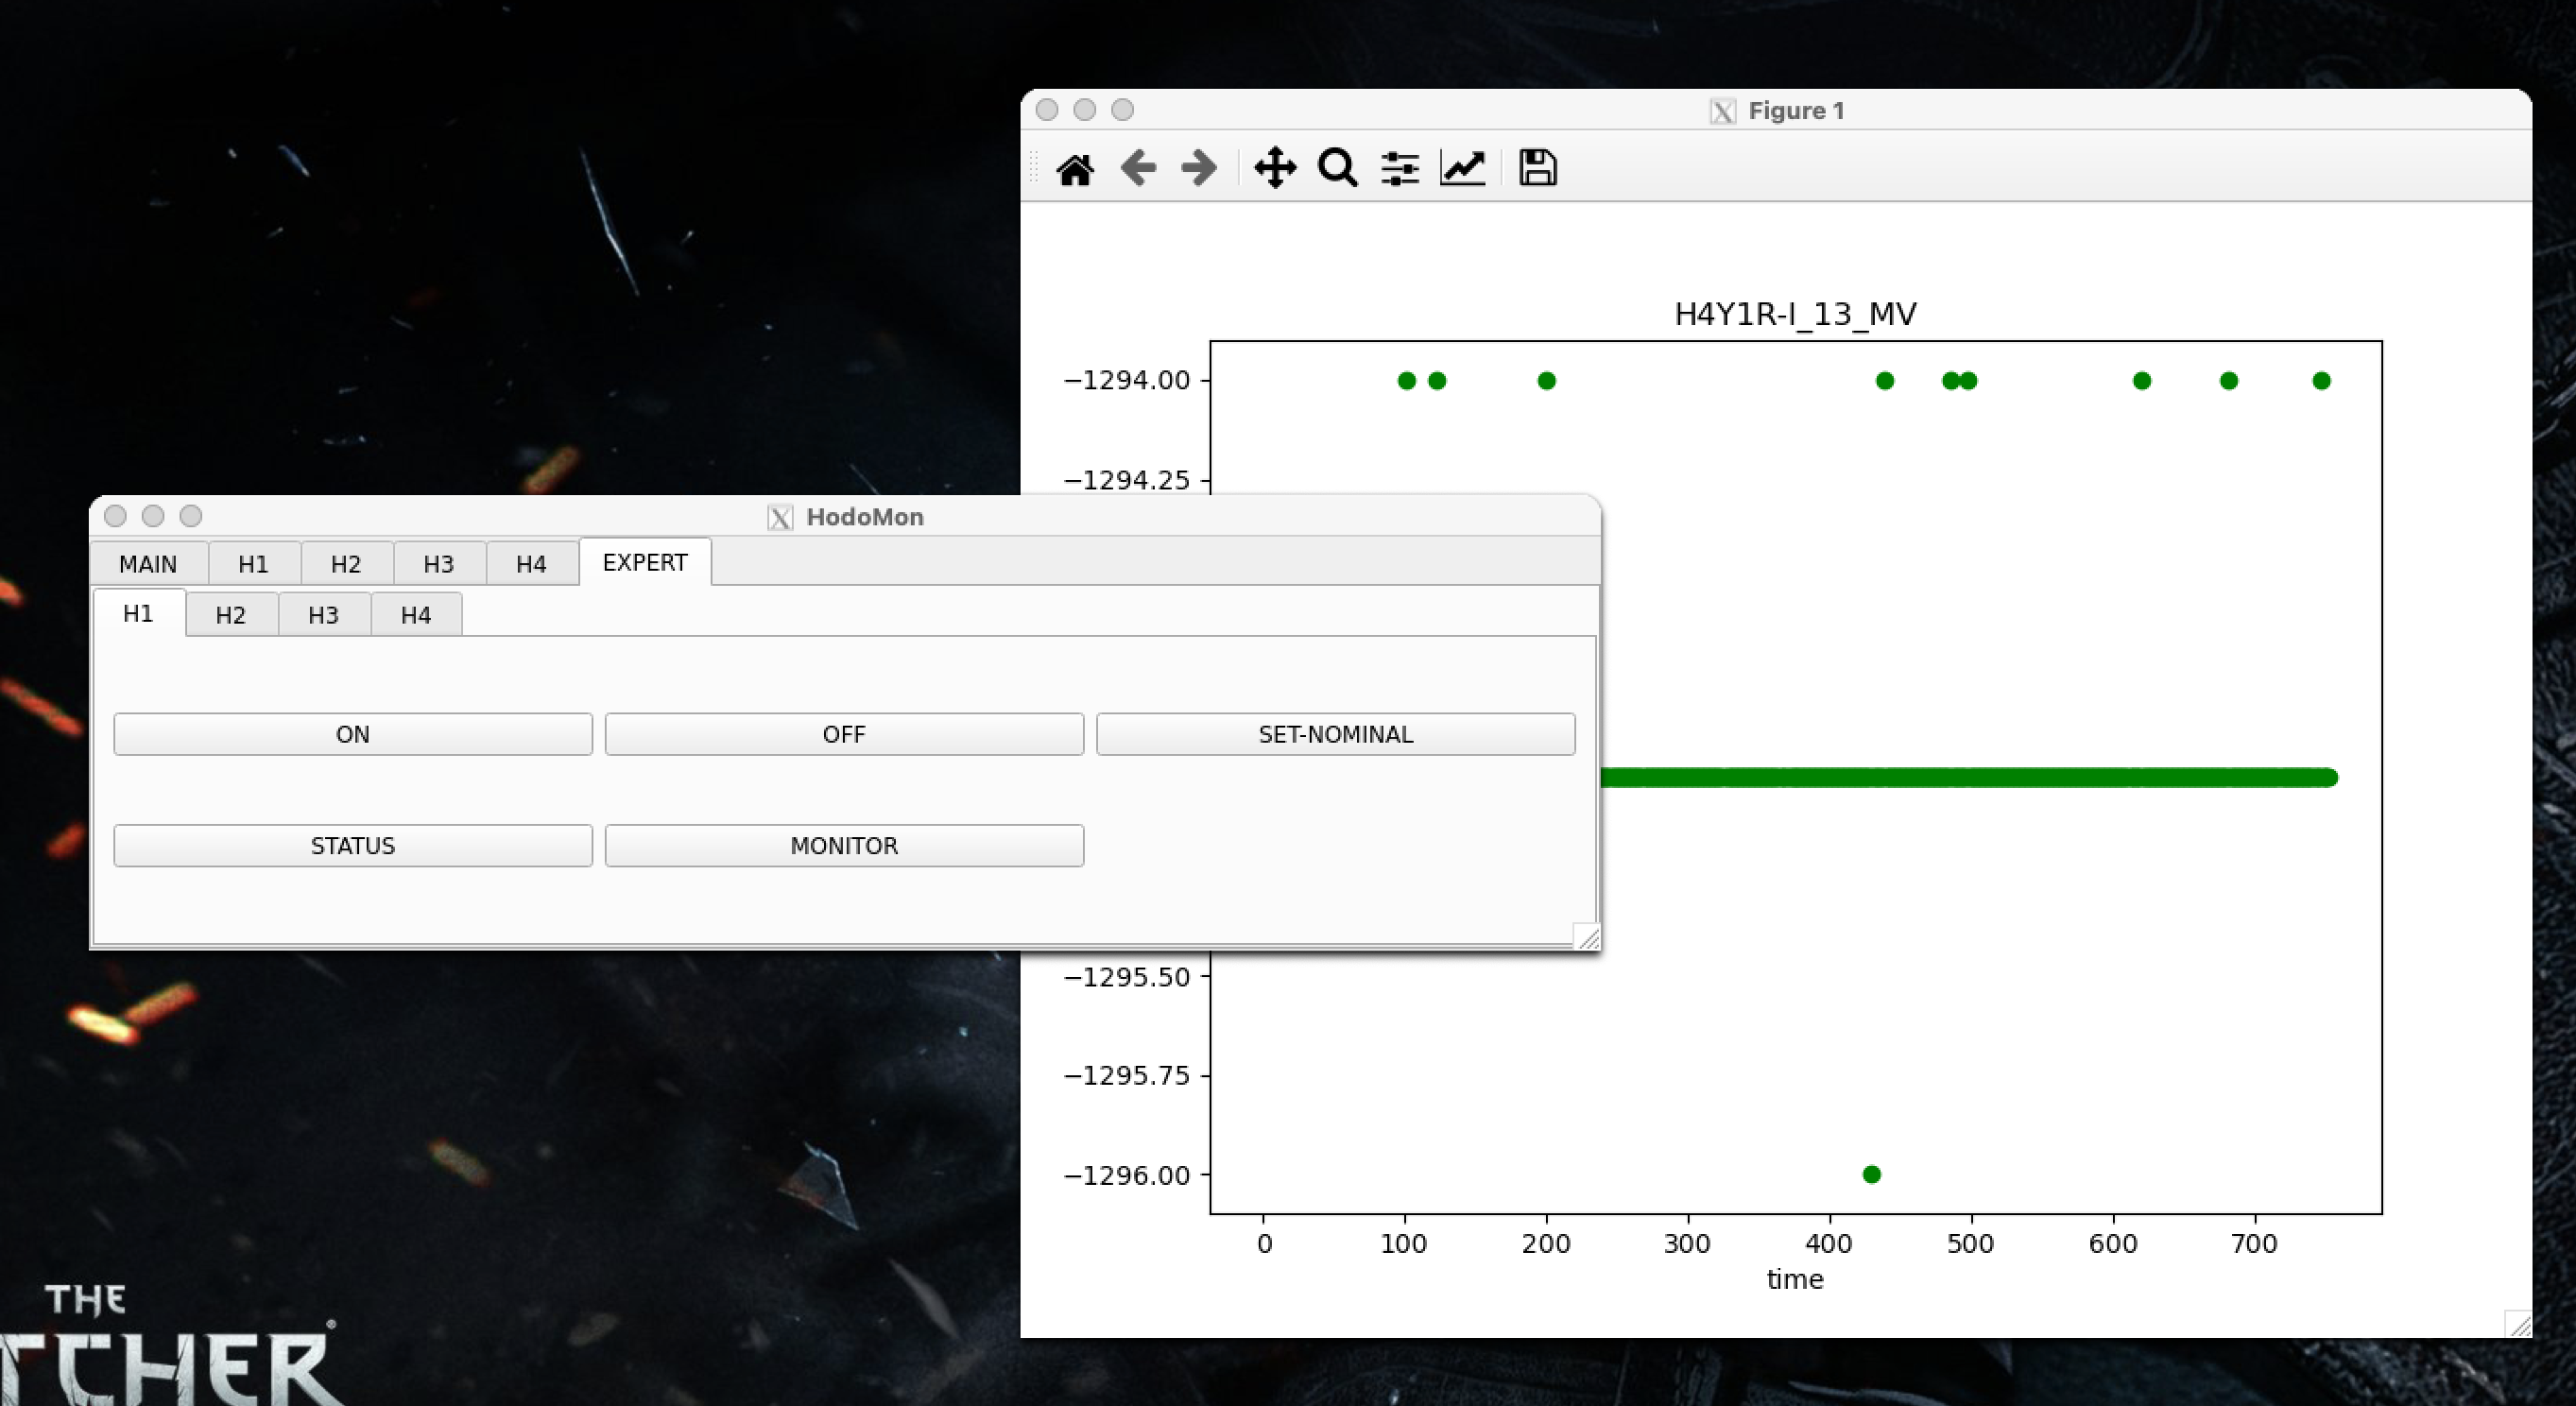
\includegraphics[width=9.0cm]{imgs/hodo_mon.png}
  \caption{Hodoscope monitoring GUI.}
\end{Pic}
\end{frame}

\begin{frame}[fragile]{Plan for Spectrometer Commissioning}
\begin{List}{15.0}{(0.5, 2.5)}

  \item We plan to fine tune the detector efficiencies during the spectrometer commissioning.

  \item For this we plan to use 4 fold trigger similar to \verb|NIM1|.

  \item We have prepared a handbook for Hodoscope/NIM subsystem. This can be used during the shifts. \href{https://github.com/dinupa1/NIM_Hodo_Handbook/blob/main/NIM_Hodo_Handbook.pdf}{Link}

  \item We have developed software to calculate hodoscope efficiencies and remote debugging.

\end{List}
\end{frame}

\end{document}